\chapter{Dynamic analysis}

\section{Legend}
	\begin{figure}[ht]
			\begin{center}
				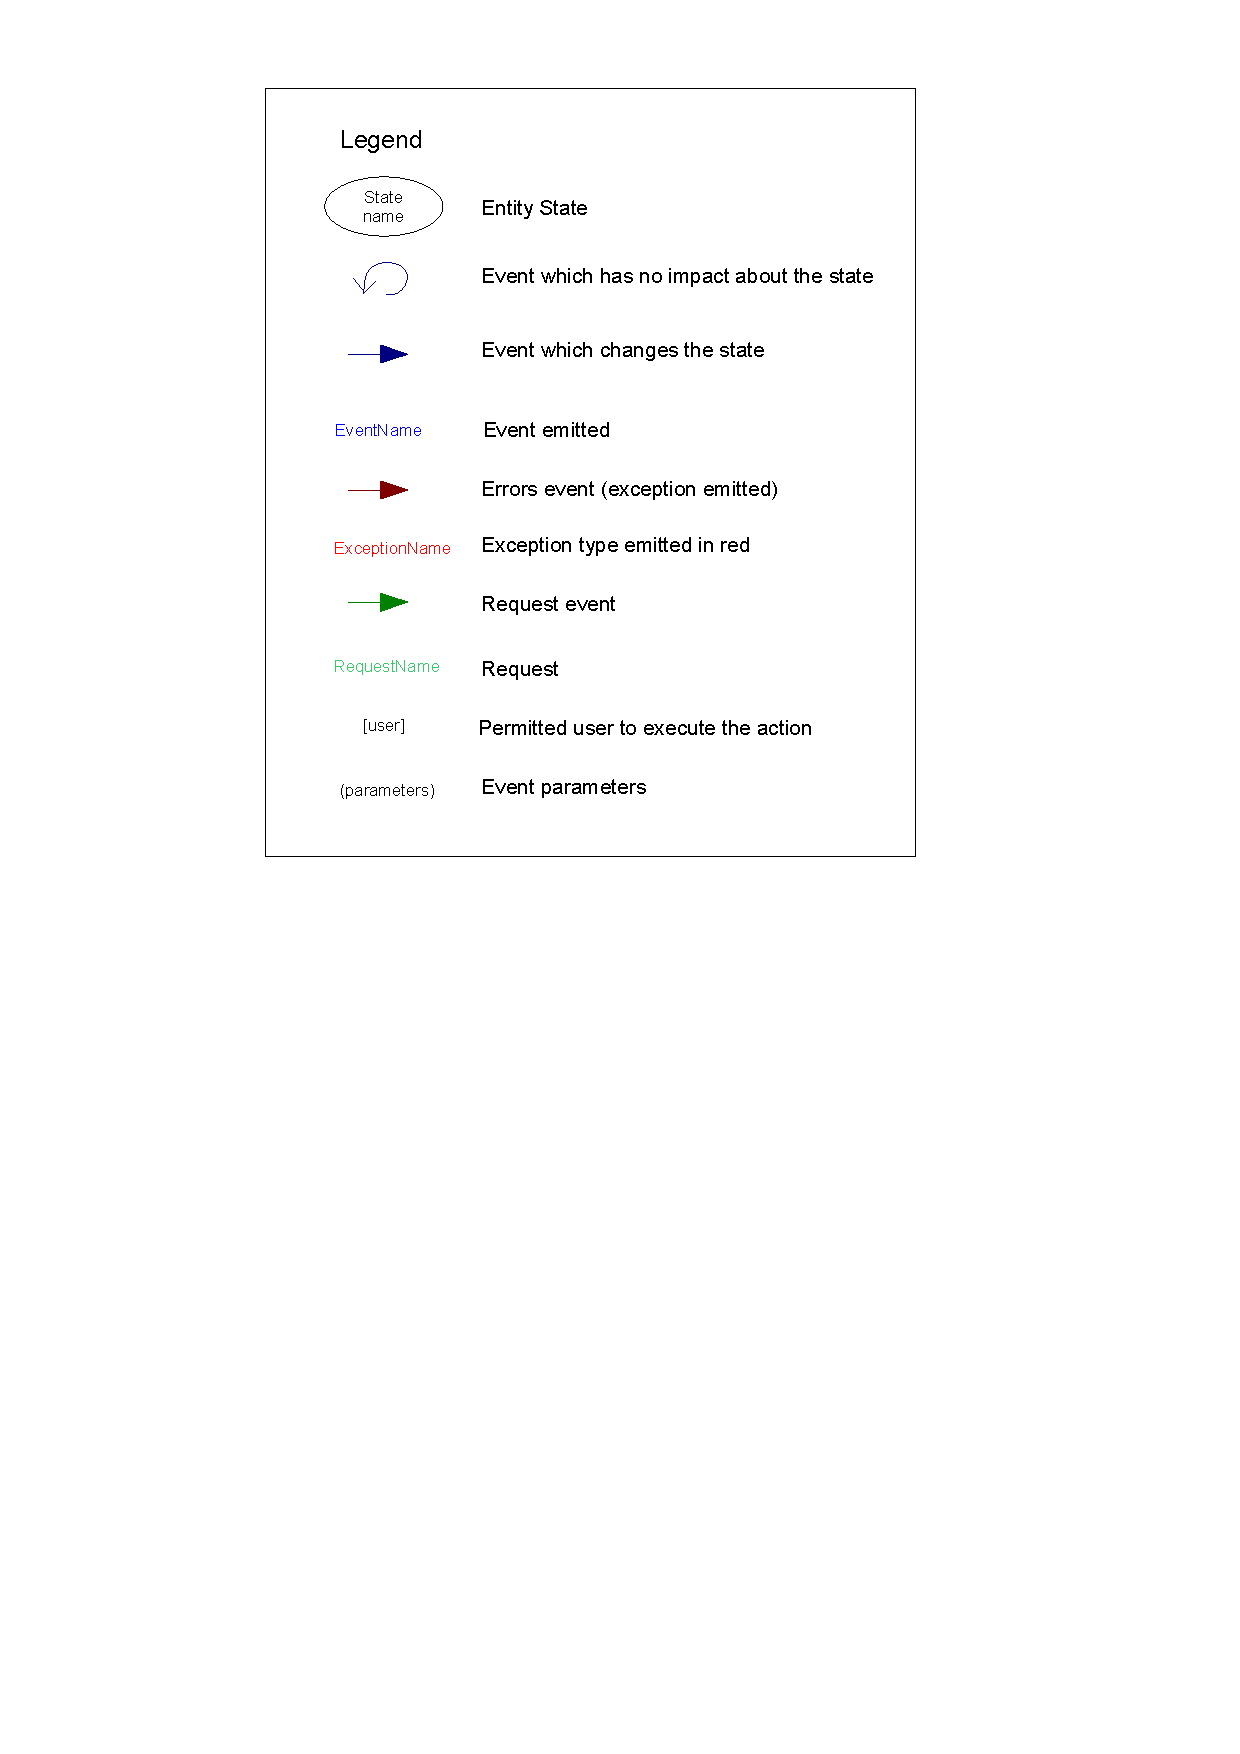
\includegraphics[width=\textwidth,  trim=2cm 14cm 2cm 1cm]{UML_figure/state_transition/dojo_logic/st_legend.pdf}
				\caption{Legend for state transition diagram}
			\end{center}
	\end{figure}
\newpage
\section{User}
	\begin{figure}[ht]
			\begin{center}
				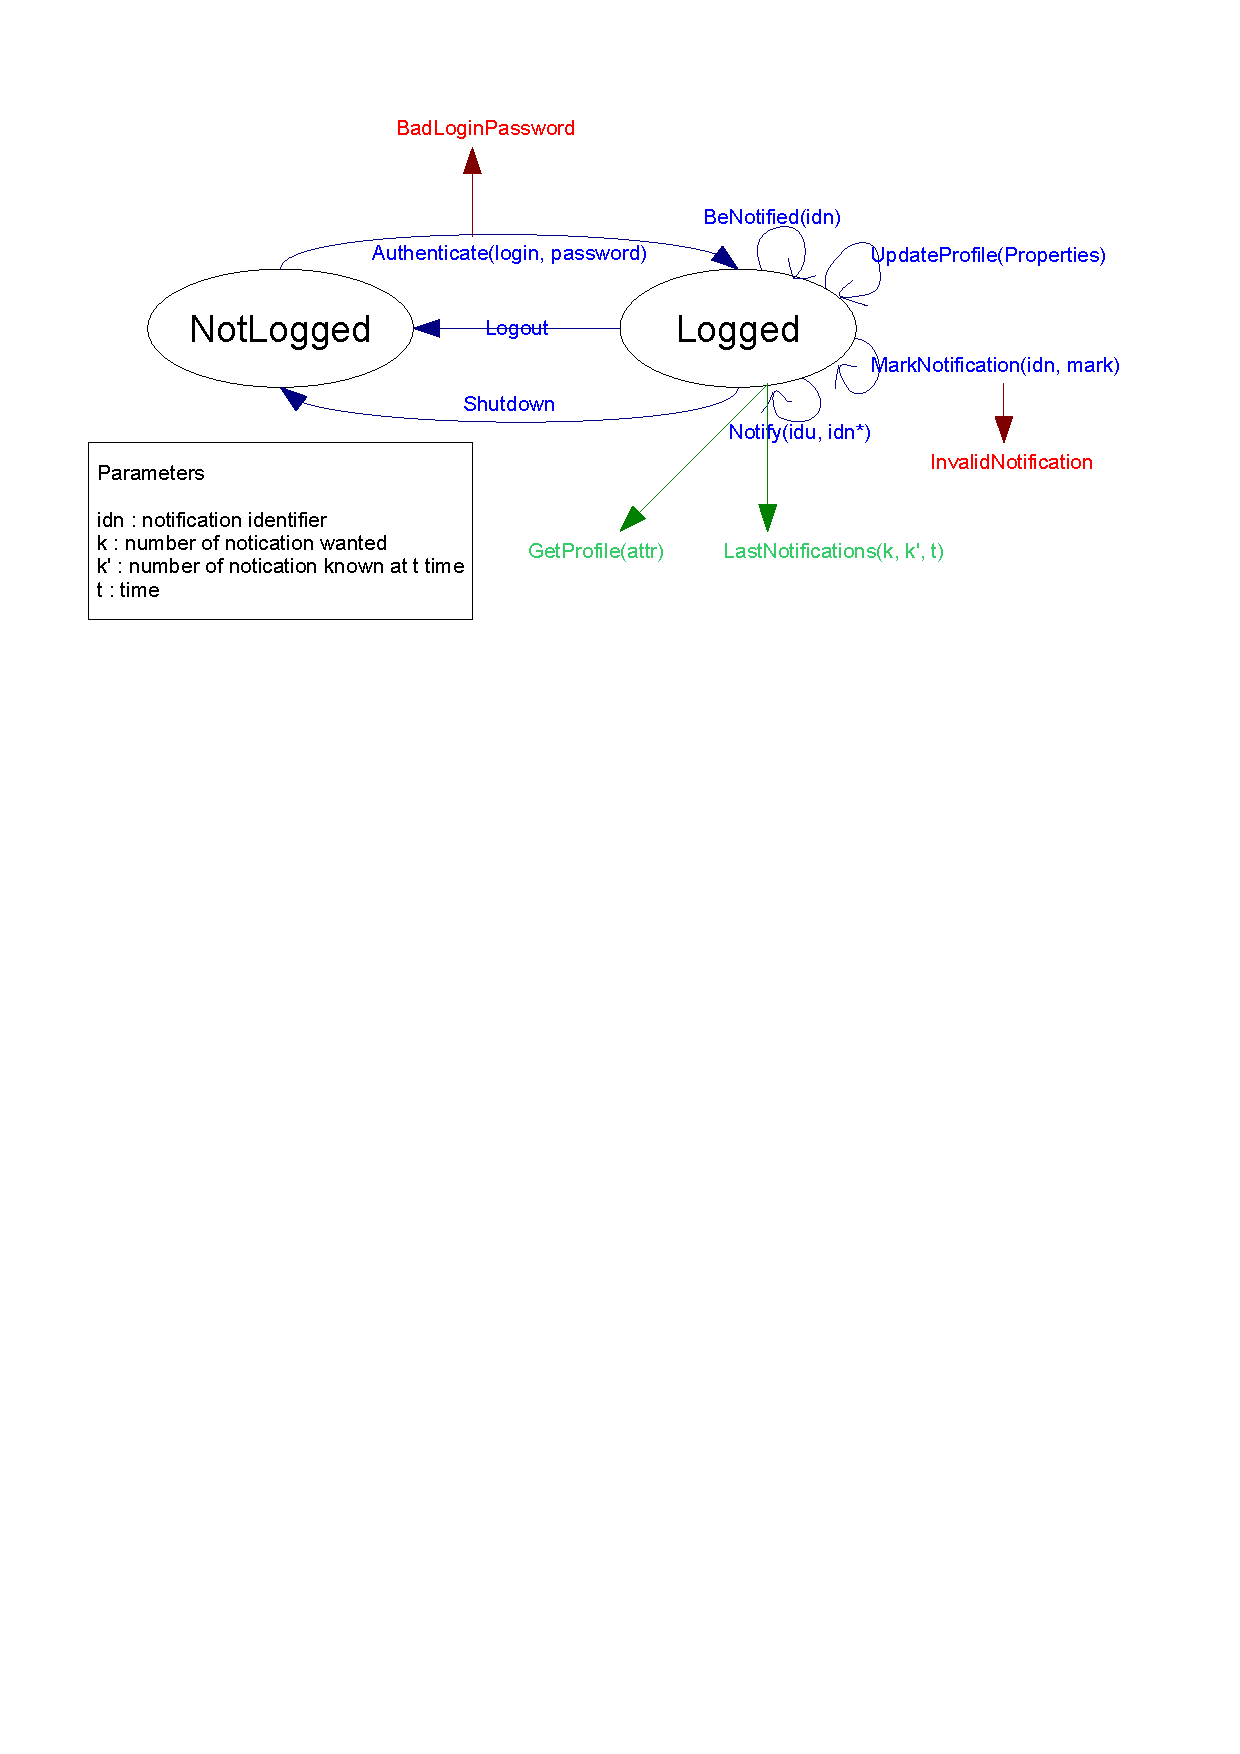
\includegraphics[width=\textwidth,  trim=2cm 18cm 2cm 1cm]{UML_figure/state_transition/dojo_logic/st_user.pdf}
				\caption{User state transition diagram}
			\end{center}
	\end{figure}
	\subsection{States}
		\subsubsection{Not logged}
			This state represents user which is not logged, the unidentified user.
		\subsubsection{Logged}
			This state represents user which is logged, the identified user.
	\subsection{Event : state modifier}
		\subsubsection{Authenticate}
			This event asks by an unidentified user, can produce error and does not change the actual state.
		\subsubsection{Logout}
			This event asks by an identified user for login out.
		\subsubsection{Shutdown}
			This event pushes by the platform to log out all identified user.
	\subsection{Event : state keeper}
		\subsubsection{Be notified}
			This event notifies a logged user for new messages.
		\subsubsection{UpdateProfile}	
			This event updates the profile of logged user with new properties.
		\subsubsection{Mark Notification}
			This event marks a notification received, can produce error when the notification does not exist.
		\subsubsection{Notify}
	\subsection{Request}
		\subsubsection{GetProfile}
			This request retrieves user data profile.
		\subsubsection{LastNotification}
			This request retrieves last notifications since time t and k the number of wanted notification.
	\subsection{Errors}
		\subsubsection{BadLoginPassword}
			This error is thrower when the login or the password are incorrect.
\newpage
\section{Group}
	\begin{figure}[ht]
			\begin{center}
				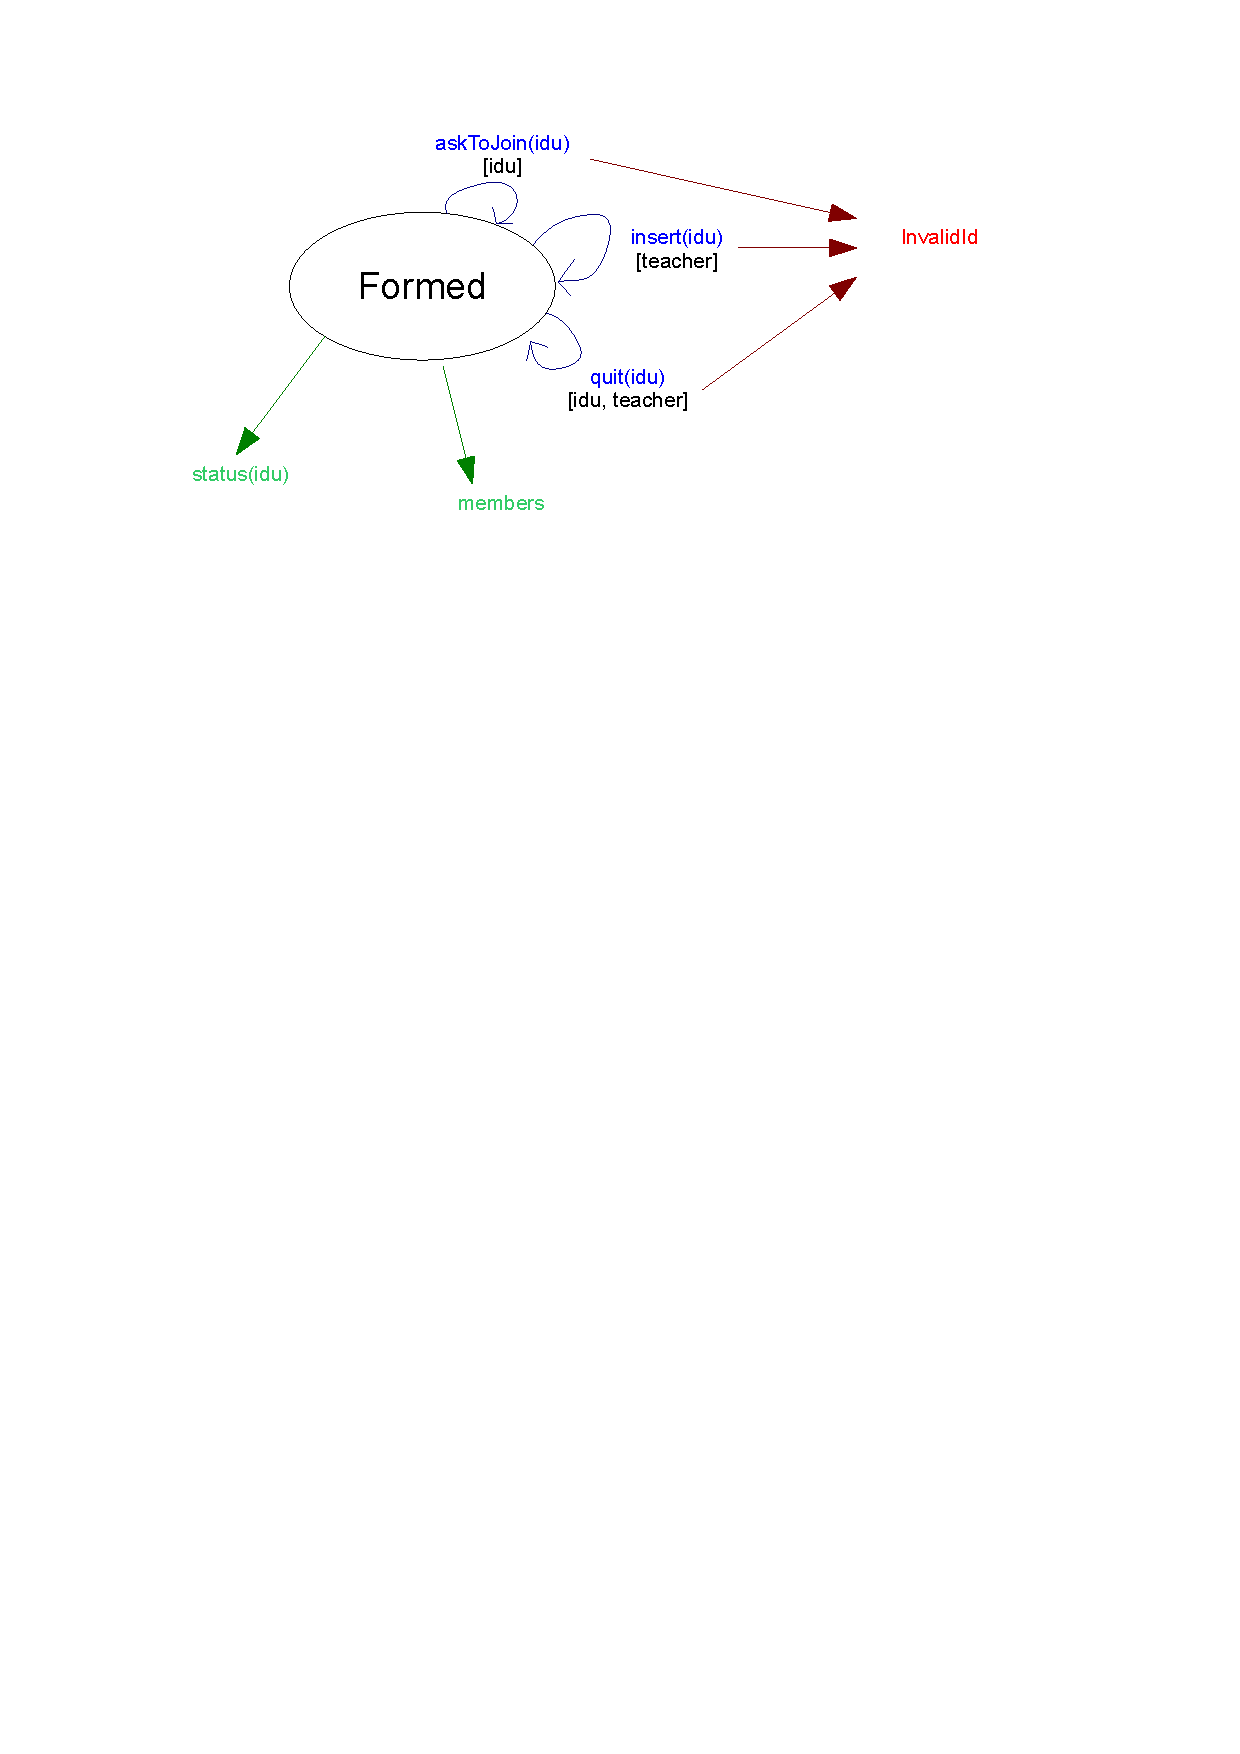
\includegraphics[width=\textwidth,  trim=2cm 18cm 2cm 1cm]{UML_figure/state_transition/dojo_logic/st_group.pdf}
				\caption{Group state transition diagram}
			\end{center}
	\end{figure}
	\subsection{States}
		\subsubsection{Formed}
			This state represents a formed group.
	\subsection{Event : state keeper}
		\subsubsection{AskToJoin}
			This event asks by an identified user to join the group, can produce error when the user is already in a waiting list.
		\subsubsection{Insert}
			This event inserts an identified user to the group, only used by teacher user.
		\subsubsection{Quit}
			This event formulated by a member from the group or a teacher to leave the group.
	\subsection{Request}
		\subsubsection{Status}
			This request retrieves the status of each members.
		\subsubsection{Members}
			This request retrieves the group members.
	\subsection{Errors}
		\subsubsection{InvalidId}
			This error is throwed when the user cannot execute these event.
\newpage
\section{Exercise}
	\begin{figure}[ht]
			\begin{center}
				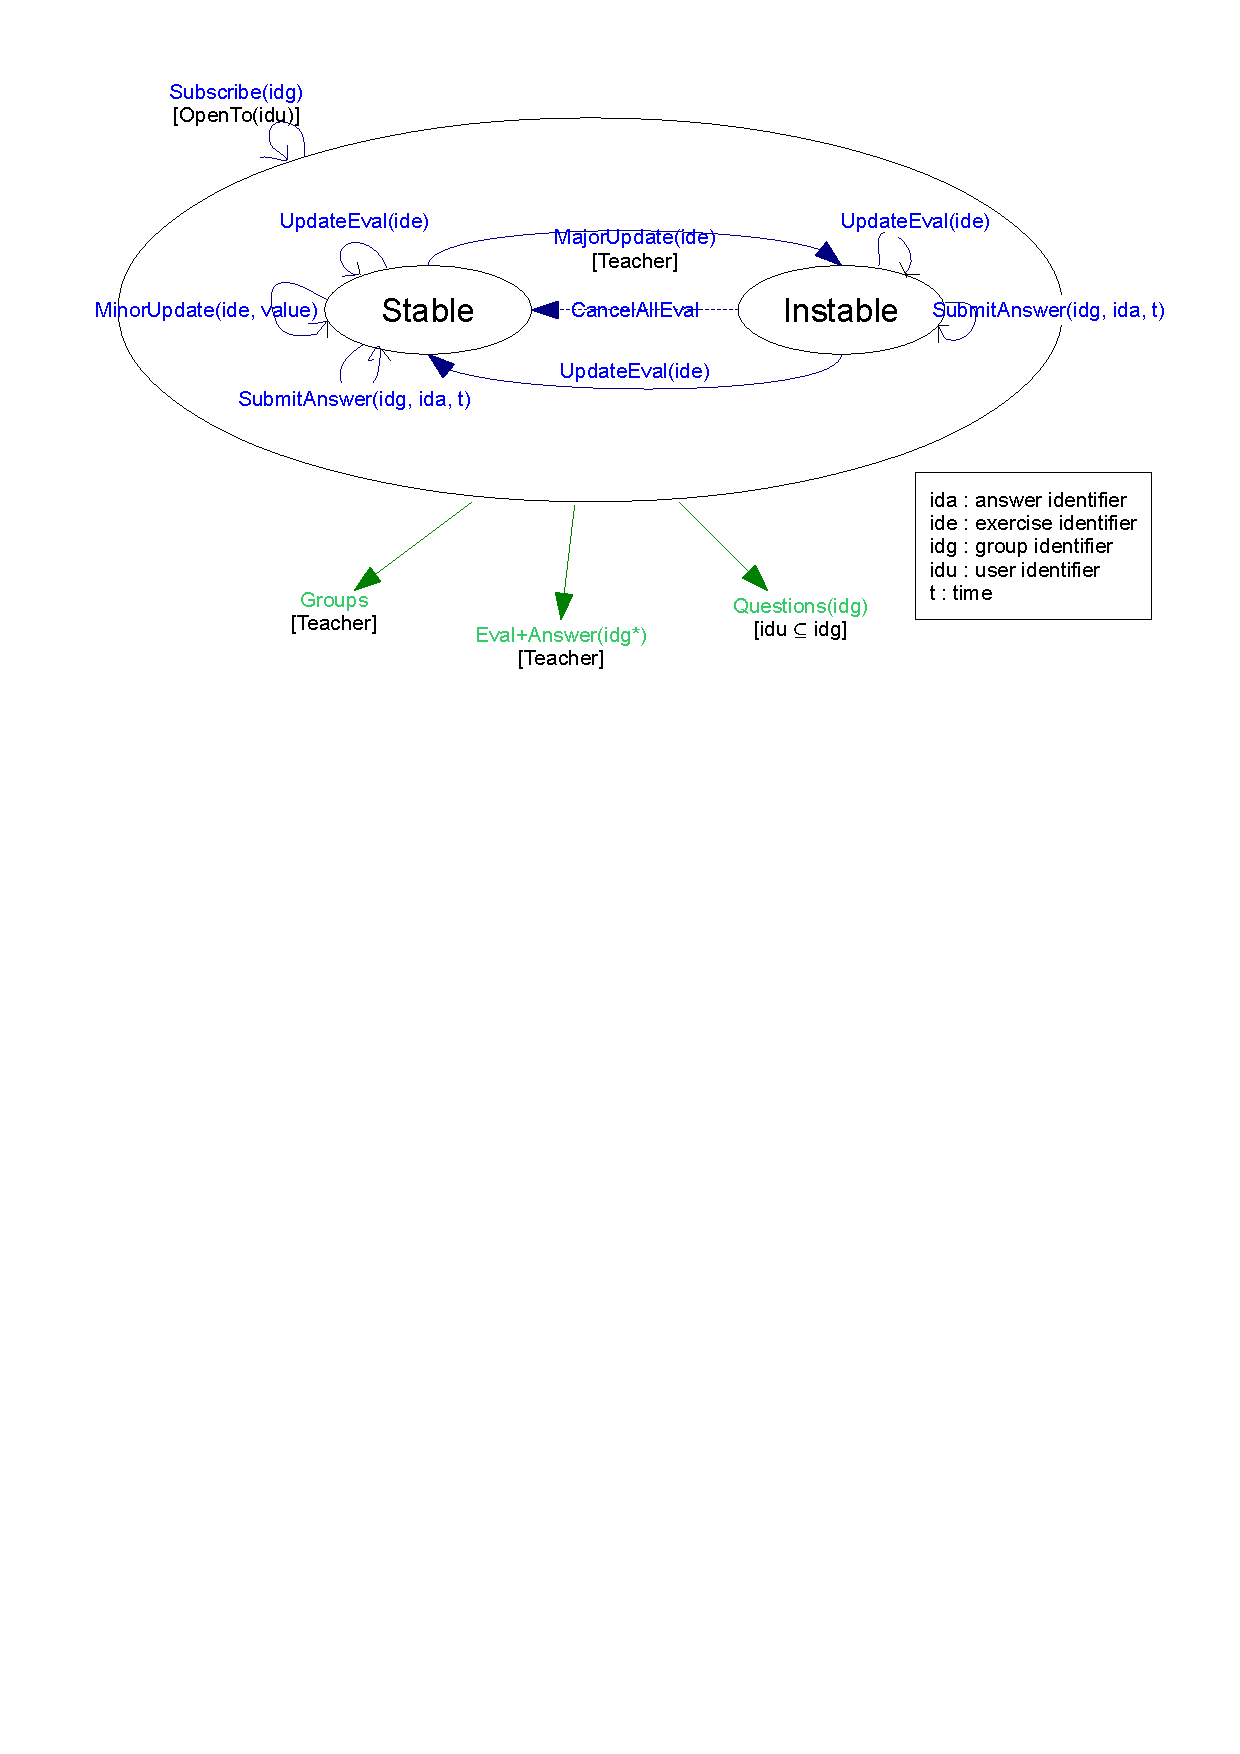
\includegraphics[width=\textwidth,  trim=2cm 18cm 2cm 1cm]{UML_figure/state_transition/dojo_logic/st_exercise.pdf}
				\caption{Exercise state transition diagram}
			\end{center}
	\end{figure}
	\subsection{States}
		\subsubsection{Stable}
			This state represents the stable version of an exercise, the exercise correction has not changed meaning the evaluation system has not changed.
		\subsubsection{Unstable}
			This state represents an exercise which undergo a major update, the exercise correction is altered with the evaluation system.
	\subsection{Event : state modifier}
		\subsubsection{MajorUpdate}
			This event is called when the evaluation method for an exercise has to change, for instance changing a coding question by a free question.
		\subsubsection{CancelAllEval}
			This event is called by the platform or the administrator meaning that all exercises which being evaluated have to be cancelled.
		\subsubsection{UpdateEval}
			This event is called when the evaluation method has not changed since a period.
	\subsection{Event : state keeper}
		\subsubsection{UpdateEval}
			This event is called when the evaluation 
		\subsubsection{MinorUpdate} 	
			This event is called when the teacher do a minor update for an exercise.
		\subsubsection{SubmitAnswer}
			This event is called when an answer is submitted.
	\subsection{Request}
		\subsubsection{Groups}
			This request retrieves group datas doing this exercise.
		\subsubsection{Eval+Answer}
			This request retrieves evaluation and answer for a group doing this exercise.
		\subsubsection{Questions}
			This request retrieves questions from the exercise for the user belonging to a group.



